\documentclass[12pt,letterpaper]{article}
\usepackage{graphicx,textcomp}
\usepackage{natbib}
\usepackage{setspace}
\usepackage{fullpage}
\usepackage{color}
\usepackage[reqno]{amsmath}
\usepackage{amsthm}
\usepackage{fancyvrb}
\usepackage{amssymb,enumerate}
\usepackage[all]{xy}
\usepackage{endnotes}
\usepackage{lscape}
\newtheorem{com}{Comment}
\usepackage{float}
\usepackage{hyperref}
\newtheorem{lem} {Lemma}
\newtheorem{prop}{Proposition}
\newtheorem{thm}{Theorem}
\newtheorem{defn}{Definition}
\newtheorem{cor}{Corollary}
\newtheorem{obs}{Observation}
\usepackage[compact]{titlesec}
\usepackage{dcolumn}
\usepackage{tikz}
\usetikzlibrary{arrows}
\usepackage{multirow}
\usepackage{xcolor}
\newcolumntype{.}{D{.}{.}{-1}}
\newcolumntype{d}[1]{D{.}{.}{#1}}
\definecolor{light-gray}{gray}{0.65}
\usepackage{url}
\usepackage{listings}
\usepackage{color}


\definecolor{codegreen}{rgb}{0,0.6,0}
\definecolor{codegray}{rgb}{0.5,0.5,0.5}
\definecolor{codepurple}{rgb}{0.58,0,0.82}
\definecolor{backcolour}{rgb}{0.95,0.95,0.92}

\lstdefinestyle{mystyle}{
	backgroundcolor=\color{backcolour},   
	commentstyle=\color{codegreen},
	keywordstyle=\color{magenta},
	numberstyle=\tiny\color{codegray},
	stringstyle=\color{codepurple},
	basicstyle=\footnotesize,
	breakatwhitespace=false,         
	breaklines=true,                 
	captionpos=b,                    
	keepspaces=true,                 
	numbers=left,                    
	numbersep=5pt,                  
	showspaces=false,                
	showstringspaces=false,
	showtabs=false,                  
	tabsize=2
}
\lstset{style=mystyle}
\newcommand{\Sref}[1]{Section~\ref{#1}}
\newtheorem{hyp}{Hypothesis}

\title{Problem Set 2}
\date{Due: February 19, 2023}
\author{Samanta Nedzinskaite}


\begin{document}
	\maketitle
	\section*{Instructions}
	\begin{itemize}
		\item Please show your work! You may lose points by simply writing in the answer. If the problem requires you to execute commands in \texttt{R}, please include the code you used to get your answers. Please also include the \texttt{.R} file that contains your code. If you are not sure if work needs to be shown for a particular problem, please ask.
		\item Your homework should be submitted electronically on GitHub in \texttt{.pdf} form.
		\item This problem set is due before 23:59 on Sunday February 19, 2023. No late assignments will be accepted.
	%	\item Total available points for this homework is 80.
	\end{itemize}

	
	%	\vspace{.25cm}
	
%\noindent In this problem set, you will run several regressions and create an add variable plot (see the lecture slides) in \texttt{R} using the \texttt{incumbents\_subset.csv} dataset. Include all of your code.

	\vspace{.25cm}
%\section*{Question 1} %(20 points)}
%\vspace{.25cm}
\noindent We're interested in what types of international environmental agreements or policies people support (\href{https://www.pnas.org/content/110/34/13763}{Bechtel and Scheve 2013)}. So, we asked 8,500 individuals whether they support a given policy, and for each participant, we vary the (1) number of countries that participate in the international agreement and (2) sanctions for not following the agreement. \\

\noindent Load in the data labeled \texttt{climateSupport.csv} on GitHub, which contains an observational study of 8,500 observations.

\begin{itemize}
	\item
	Response variable: 
	\begin{itemize}
		\item \texttt{choice}: 1 if the individual agreed with the policy; 0 if the individual did not support the policy
	\end{itemize}
	\item
	Explanatory variables: 
	\begin{itemize}
		\item
		\texttt{countries}: Number of participating countries [20 of 192; 80 of 192; 160 of 192]
		\item
		\texttt{sanctions}: Sanctions for missing emission reduction targets [None, 5\%, 15\%, and 20\% of the monthly household costs given 2\% GDP growth]
		
	\end{itemize}
	
\end{itemize}

\newpage
\noindent Please answer the following questions:

\begin{enumerate}
	\item
	Remember, we are interested in predicting the likelihood of an individual supporting a policy based on the number of countries participating and the possible sanctions for non-compliance.
	\begin{enumerate}
		\item [] Fit an additive model. Provide the summary output, the global null hypothesis, and $p$-value. Please describe the results and provide a conclusion.
		%\item
		%How many iterations did it take to find the maximum likelihood estimates?
	\end{enumerate}
	
	\lstinputlisting[language=R, firstline=39,lastline=63]{PS2.R} 

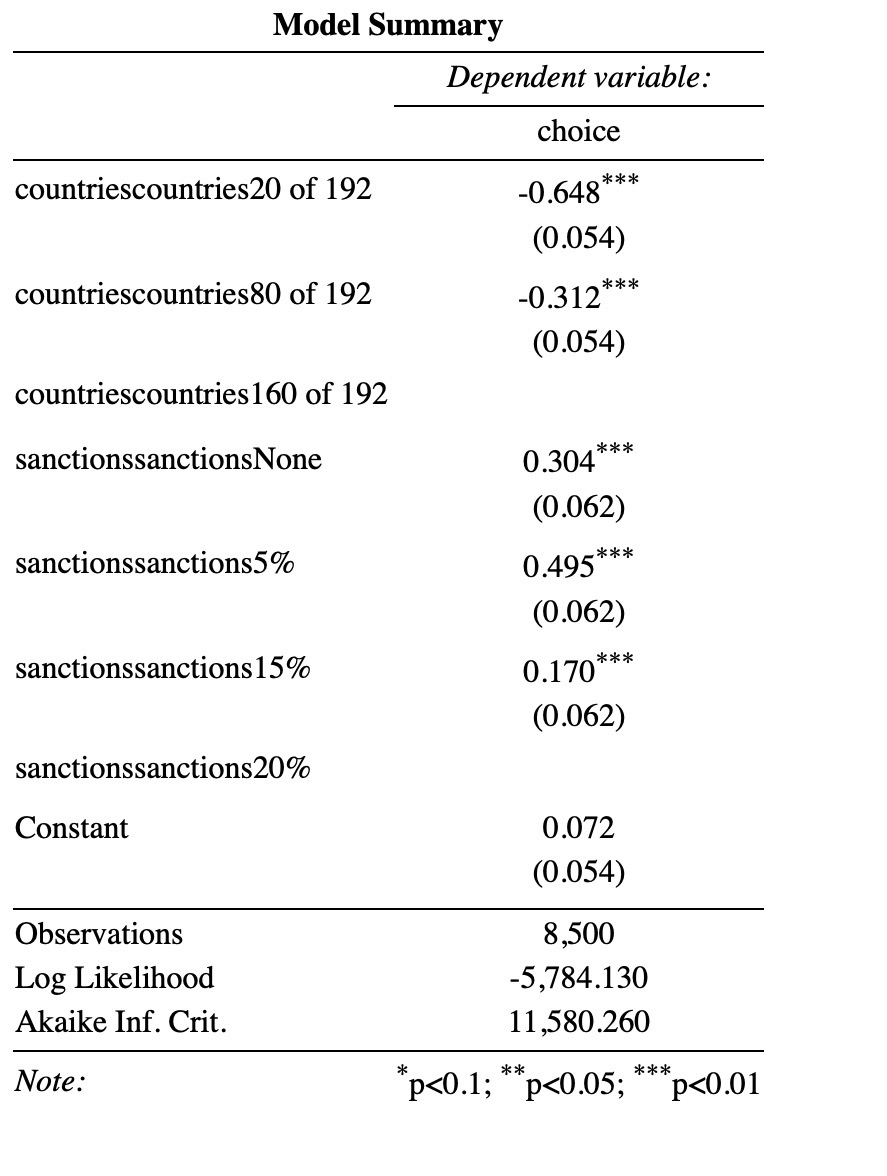
\includegraphics[width=0.8\textwidth]{model_summary.jpg}
\linebreak
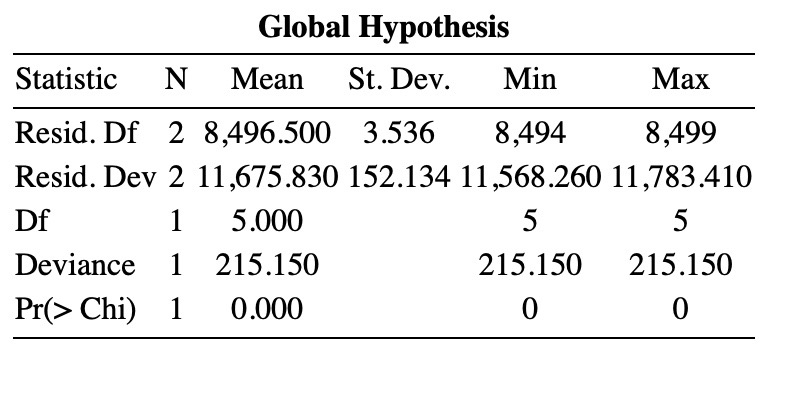
\includegraphics[width=0.8\textwidth]{global_hypothesis.jpg}
\linebreak
\textbf{The p-value s is 0.000, which is less than the significance level of 0.05, providing good evidence against the null hypothesis, that the observed data fits the predicted distribution very well. }

The countries variable has three dummy variables, with the reference category being 192 of 192. The coefficients for countries20 of 192 and countries80of192 are negative and statistically significant, which means that compared to 192of192 countries, the odds of supporting the policy are lower for individuals from countries that participated in the policy to a lesser extent (i.e., 20 or 80 out of 192 countries). 

The sanctions variable has four dummy variables, with the reference category being sanctionsNone. The coefficients for sanctions5 and sanctions15 are positive and statistically significant, which means that compared to having no sanctions, the odds of supporting the policy increase when the sanctions are set to 5 percent and 15 percent of the monthly household costs (given 2 percent GDP growth) (as opposed to having no sanctions in place)

\textbf{Drawing a conclusion from the results of the model analysis, it can be said that both the countries and sanctions variables have a statistically significant effect on an individual's likelihood of supporting the policy. Individuals from countries that participated in the policy to a lesser extent (i.e., 20 or 80 out of 192 countries) compared to those from countries that participated more (i.e., 160 out of 192) are less likely to support the policy. Additionally, the odds of supporting the policy increase when the sanctions are set to 5 percent and 15 percent of the monthly household costs (given 2 percent GDP growth).}
	\item
	If any of the explanatory variables are significant in this model, then:
	\begin{enumerate}
		\item
		For the policy in which nearly all countries participate [160 of 192], how does increasing sanctions from 5\% to 15\% change the odds that an individual will support the policy? (Interpretation of a coefficient)
%		\item
%		For the policy in which very few countries participate [20 of 192], how does increasing sanctions from 5\% to 15\% change the odds that an individual will support the policy? (Interpretation of a coefficient)

\vspace{.8cm}
	\textbf{As can be seen from the summary output, the difference between the coefficients for sanctionssanctions15 (0.170) and sanctionssanctions5 (0.495) is 0.325. This means that when the sanction level increases from 5 percent to 15 percent, the log odds of supporting the policy increase by 0.325.}
\vspace{.8cm}
		\item
		What is the estimated probability that an individual will support a policy if there are 80 of 192 countries participating with no sanctions? 
		\vspace{.8cm}
		
\textbf{\textbf{We can find the estimated probability using this formula:}	log(p / (1 - p)) = b0 + b1X1 + b2X2 + bk*Xk} 
or the inverse \textbf{p = 1 / [1 + exp(- (b0 + b1X1 + b2X2 + ... + bk*Xk))]}
		\lstinputlisting[language=R, firstline=89,lastline=92]{PS2.R} 

0.4800107

\textbf{The estimated probability that an individual will support the policy if there are 80of192 countries participating with no sanctions is 0.48/48 percent.}
\vspace{.8cm}
		\item
		Would the answers to 2a and 2b potentially change if we included the interaction term in this model? Why? 
		\begin{itemize}
			\item Perform a test to see if including an interaction is appropriate.
		\end{itemize}
		\lstinputlisting[language=R, firstline=74,lastline=80]{PS2.R} 
		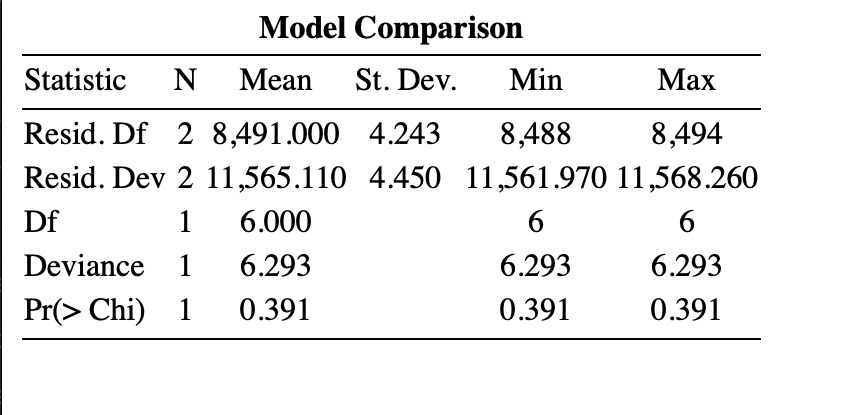
\includegraphics[width=0.8\textwidth]{model_comparison.jpg}
		\linebreak
As we can see from the table above, the p-value is 0.3912, which is much greater than the significance level of 0.05. As a result, there is not great evidence to suggest that Model 2 with the interaction termis a better fit for the data than Model 1 with only the effects added together. 
	
	\end{enumerate}
	\end{enumerate}


\end{document}
